
% Document class: article with font size 11pt
% ---------------
\documentclass[11pt,a4paper]{report}

% Call packages
% ---------------
\usepackage{comment} %Possible to comment larger sections
%http://get-software.net/macros/latex/contrib/comment/comment.pdf
\usepackage[T1]{fontenc} %oriented to output, that is, what fonts to use for printing characters.
\usepackage[utf8]{inputenc} %allows the user to input accented characters directly from the keyboard
%Put fontenc before inputenc
\usepackage{fourier} %Better typeface
%http://mirrors.dotsrc.org/ctan/fonts/fourier-GUT/doc/latex/fourier/fourier-doc-en.pdf
\usepackage[danish]{babel}														     % Danish
\usepackage[protrusion=true,expansion=true]{microtype}				                 % Better typography
%http://www.khirevich.com/latex/microtype/
\usepackage{amsmath,amsfonts,amsthm, amssymb}							 % Math packages
\usepackage[pdftex]{graphicx} %puts to pdf and graphic
%http://www.kwasan.kyoto-u.ac.jp/solarb6/usinggraphicx.pdf
\usepackage{xcolor,colortbl}
%http://mirrors.dotsrc.org/ctan/macros/latex/contrib/xcolor/xcolor.pdf
%http://texdoc.net/texmf-dist/doc/latex/colortbl/colortbl.pdf
\usepackage{tikz} %documentation http://www.ctan.org/pkg/pgf
\usepackage{parskip} %http://www.ctan.org/pkg/parskip
%http://tex.stackexchange.com/questions/51722/how-to-properly-code-a-tex-file-or-at-least-avoid-badness-10000
%Never use \\ but instead press "enter" twice. See second website for more info
\usepackage{empheq}
\usepackage{caption}
\usepackage{tablefootnote}
\usepackage{natbib}
\usepackage{listings}
\usepackage{pdfpages}

\usepackage[all,dvips,line]{xy} %Arrows and text in math

\usepackage{float}

\usepackage{hyperref} %Til at vise links i pdf filen så man kan hoppe frem og tilbage
\hypersetup{
    colorlinks,
    linkcolor={blue!35!black},
    citecolor={blue!50!black},
    urlcolor={blue!80!black}
}


% MATH -------------------------------------------------------------------
\newcommand{\Real}{\mathbb R}
\newcommand{\Complex}{\mathbb C}
\newcommand{\Field}{\mathbb F}
\newcommand{\RPlus}{[0,\infty)}
%
\newcommand{\norm}[1]{\left\Vert#1\right\Vert}
\newcommand{\essnorm}[1]{\norm{#1}_{\text{\rm\normalshape ess}}}
\newcommand{\abs}[1]{\left\vert#1\right\vert}
\newcommand{\set}[1]{\left\{#1\right\}}
\newcommand{\seq}[1]{\left<#1\right>}
\newcommand{\eps}{\varepsilon}
\newcommand{\To}{\longrightarrow}
\newcommand{\RE}{\operatorname{Re}}
\newcommand{\IM}{\operatorname{Im}}
\newcommand{\Poly}{{\cal{P}}(E)}
\newcommand{\EssD}{{\cal{D}}}
% THEOREMS ----------------------------------------------------------------
\theoremstyle{plain}
\newtheorem{thm}{Theorem}[section]
\newtheorem{cor}[thm]{Corollary}
\newtheorem{lem}[thm]{Lemma}
\newtheorem{prop}[thm]{Proposition}
%
\theoremstyle{definition}
\newtheorem{defn}{Definition}[section]
%
\theoremstyle{remark}
\newtheorem{rem}{Remark}[section]
%
\numberwithin{equation}{section}
\renewcommand{\theequation}{\thesection.\arabic{equation}}


\begin{document}

\textbf{Rettelser:}
Tegninger til alle!!

\textbf{Divide and Conquer:}\\
Bedre intro til Divide and Conquer

Quicksort skrevet ud

Closest pair of points

\textbf{Priority Queues and Heaps:}\\
Priority queues forkortet og skrevet præcist

Algoritme til Max-Heapify

Køretid, tilføj O notation

\textbf{Binary-Search-Trees:}\\
Notation fejl i Lemma 13.1

Ændre tekst når højde skal påvises til mere intuitivt

\textbf{Dynamic Programming:}\\

\textbf{Greedy Algorithm:}\\
Lemma 16.2 tilføj rettelse til beviset

\textbf{Minimum Spanning Trees:}\\
Korrekthed for Kruskal og Køretid

Korrekthed for Prim og Køretid

\textbf{Shortest Path:}\\
Intro

Negative-weight edges s.645

S.650 info

Intro til lemma 24.1

\newpage


\tableofcontents

\newpage

\chapter{Divide and Conquer S. 65}

\section{Definition}
Bruges til at løse rekursive problemer. For at kunne løse et problem, skal det udvise optimale substukture. Hvis man bruger bruteforce vil tiden være $n^2$, men ved D'n'C ender man med $n \log n$

\section{Divide and Conquer s. 65}

\begin{enumerate}
  \item Divide: Opdel problemet mindre delproblemer, gør dette til vi har trivielle problemer.
  \item Conquer: Fin lokalt optimale løsning til alle delproblemer.
  \item Combine: Kombiner delløsninger til en global løsning
\end{enumerate}

\section{MERGE-SORT}

Antag man har en liste (1, 2, 3, 5, 2, 8, 3, 1) den deles op i to.


Altså har vi (1, 2, 3, 5) og (2, 8, 3, 1). Dette deles op (1, 2), (3, 5), (2, 8) og (3, 1) hvor vi ender med en sorteret liste på (1, 1, 2, 2, 3, 3, 5, 8).

Ved at analysere MERGE-SORT så
\begin{itemize}
  \item \textbf{DIVIDE} koster $\Theta(1)$
  \item \textbf{CONQUER} løser rekursivt 2 subproblemer, som hver har størrelsen n/2, som er 2T(n/2)
  \item \textbf{COMBINE} Som samler alle n-elementer som tager $\Theta(n)$ tid
\end{itemize}

\subsection{Mergesort Rekursion}
Da vi sorterer to lister i O(n log n) tid. Dernæst bliver der for hver rekursion dannet to underproblemet af størrelsen n/2 og dette sker i lineær tid. Altså fås rekursionstræet for merge sort's køretid være
\[
T(n) =  \begin{cases}
              \begin{array}{c}
                \Theta(1), \quad if n = 1 \\
                2T(n/2) + O(n), \quad if n > 1
              \end{array}
              \end{cases}
\]
\begin{enumerate}
  \item Divide: Finder snit af størrelsen af det der skal sorteres. Køretiden er $\Theta(1)$
  \item Conquer: Rekursivt løser to subproblemer med hver størrelse af n/2 som er $2T(n/2)$
  \item Combine: MERGE (samler) n-elementer som tager $\Theta(n)$ tid
\end{enumerate}

Altså løses rekursionstræet som givet ovenfor. Dvs at worst case køretid er $O(n \log n )$ og dette kan vises med substitution

Ved at kigge på rekursionstræet, så kan vi forstår hvordan det virker

\section{Rekursions træ}

\begin{figure}[H]
  \centering
  % Requires \usepackage{graphicx}
  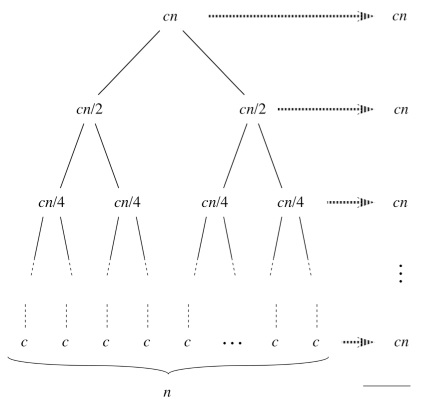
\includegraphics[scale=1]{rekursion.jpg}\\
  \caption{lg n + 1 levels med cost cn pr level. T(n) = cn(lg n) + cn = $\Theta(nlgn)$}
\end{figure}

Altså man fortsætter indtil man kommer ned til 1 problem, hvor
\begin{itemize}
  \item Top koster cn
  \item Videre ned har man 2 subproblemer som hver koster cn/2
  \item Videre ned har man 4 subproblemer som hver koster cn/4
  \item Hver gang man gå et niveau ned, så fordobles subproblemerne, men kosten halveres, derfor forbliver kosten det sammen
\end{itemize}

Da højden af træet er $\log n$, kommer vi op på den totale "cost" $T(n) = \Theta(n \log n)$

\section{Substitution}
Vi gætter en løsning og bruger induktion til at se at det virker. Ved MERGESORT: $T(n) = T(n/2) + O(n)$, så vores gæt er $T(n) \leq c n \log n$ for en konstant c > 0, $n_0 > 0$ og n > 1. Men da $\log(1) = 0$ så prøves for $2 \leq n < 4$, da $T(2)=4$ og $T(3)=5$. Så nu prøves med induktionsskridtet.
\begin{align*}
    T(n) =& 2T(n/2) + O(n) \\
    \leq& 2 c(n/2) \log(n/2) + c_1 n \\
    =&  cn \log(n/2) + c_1 n  \\
    =&  cn (\log(n) - 1) + c_1 n  \\
    =&  cn \log(n) - cn + c_1 n  \\
    =&  cn \log(n) + (c_1 - c) n  \\
\end{align*}
Hvis vi vælger et c der holder for $c \geq c_1$, så får vi at at det holder for $O(n \log n)$ og hvis det vælges at $c = c_1$, fås at det også holder for $\Theta(n \log n)$

\section{Master Theorem}
Er en generel løsning til en masse rekursive algoritmer. Hvis en rekusion har formen $T(n) = a T(n/b) + f(n)$ hvor a og b er konstanter og fn er en Theta begrænsing for køretiden på hvert rekursion, så finders der 3 cases
\begin{enumerate}
  \item Hvis $f(n) = O(n^{\log_b a - \epsilon})$ så $T(n) = \Theta(n^{\log_b a})$
  \item Hvis $f(n) = \theta(n^{\log_b a })$ så $T(n) = \Theta(n^{\log_b a}\log n)$
  \item Hvis $f(n) = \Omega(n^{\log_b a + \epsilon})$ og $a f(n/b) \leq cf(n)$ så $T(n) = \Theta(f(n))$
\end{enumerate}

\section{Quicksort S. 170}
I Quicksort algoritmen vælges for hvert rekursivt kald en pivot, hvortil partitionen subrutinen køres. Denne rutine sørger for at der i listen i lineær tid bliver opdelt i to underlister hvor pivoen er i midten, og alt mindre til venstre og alt større til højre. Hertil køres quicksort rekursivt på hhv. venstre og højre underlist.

Hvor opdelen sker er altafgørende for køretiden for quicksort er god. Quicksort har i sig selv gode konstanter og vil uanset opdeling køre i $O(n \log n)$, dog vil logaritmen have forskellig base, hvilket svare til en konstant til forskel.

\subsection{Running time}

\begin{description}
  \item[DIVIDE] Partition the array A[p .. r] into two subarrays A[p .. q - 1] and A[q + 1 .. r ]
  \item[CONQUER] Sort the two subarrays
  \item[COMBINE] The arrays are sorted, no work needed to combine
\end{description}

\section{Closest pair of points s. 1039}

\chapter{Priorty queues and Heaps s. 151}
\section{Priorty queues}
Implentere et sæt S af elementer, hvor hvert element er associeret med en nøgle (key)
\begin{itemize}
  \item \textbf{Max(S)}: Returnere max elemetet af prioritetskøren uden af fjerne den. Da det er en max-heap gøres dette i $\Theta(1)$
  \item \textbf{Extract-max(S)}:  Skal elementet fjernes gør vi ligesom i heapsort, blot med et enkelt element, holder styr på hvilket element vi sætter bagerst i vores heap og reducerer heap størrelsen med 1
  \item \textbf{Increase-key(S,x,k)}: Har vi brug for at forøge en key i vores prioriteskø er vi nødt til at lave en omvendt max-heapify, idet vi kan lave en lokal violation af en heap property. En slags "bubble up". vi tjekker om parent er mindre en vores nuværende element. Hvis ja byttes disse og vi tjekker igen ve denne parent om dens parent er mindre indtil dette ikke længere er tilfældet.
  \item \textbf{Insert(S,x)}: For at indsætte en nøgle forøges heapstørrelsen med en, elementet puttes bagerst med key $-\infty$ og der kaldes increase key på dette element med den ønskede værdi.
\end{itemize}

\section{Definition s.151-153}
Er en datastruktur hvorpå man på en systematisk måde gemmer data på. Der arbejdes med et sæt regler, hvorpå hvert "child" enten er større eller mindre end en selv, medens man bevæger sig ned.\\
En heap kan grafisk fremstilles som et graf-træ, med en top og fra hver knude højst 2 kanter.

Given en knude med indeks $i$, kan dens forældre findes ved at beregne $\lfloor i/2 \rfloor$ og dens børn ved at beregne $2i$ og $2i+1$ hhv for venstre og højre.

Så en Heap er et array visuleret som et næsten komplet binary træ.
\[
\begin{array}{cccccccccc}
  1 & 2 & 3 & 4 & 5 & 6 & 7 & 8 & 9 & 10 \\
  16 & 14 & 10 & 8 & 7 & 9 & 3 & 2 & 4 & 1
\end{array}
\]
Som det ses, så er det ikke sorteret. Indeks 1 er roden af træet.

\section{Heap Property s. 154}
Alle Heap operationer er bygget omkring en invariant ved navnet "The heap property" som altid er opfyldt efter hver operation på en Heap.

Roden af træet: Er det første element (i = 1)

\begin{itemize}
  \item Parent(i) = i/2
  \item Left(i) = 2i
  \item Right(i) = 2i + 1
\end{itemize}


\section{Max-Heapify}

Træet som tegnet før har en Max-Heap Property

\begin{itemize}
  \item \textbf{Max heap property:} $A[Parent(i)] \geq A[i]$
  \item \textbf{Min heap property:} $A[Parent(i)] \leq A[i]$
\end{itemize}


Tager en Heap A og et index i, og antager at subtræerne med rødderne

For at lave en Max-Heap vil vi gøre brug af Max-Heapify nedefra og op.

Det Max-Heapify gør: rydder op i en enkelt violation af heap property, i et subtræ's rod, se eksemplet

\section{Build-Max-Heap s. 156}
Vi kan bruge MAX-HEAPIFY med en bottom-up metode, til at lave an array A[1..n], hvor n = A.length til en max-heap. Det elementer der er i subarrayed A[(n/2)+1..n] er alle blade i træet.

Vi behøver ikke køre max-heapify på bladende ideet de allerede er en max-heap per defintion. I stedet køres max-heapify nedad fra [n/2],...,1.
For at vise at dette giver en max-heap defineres følgende invariant.

Før hver iteration ved element med index i, er alle elementer i+1, i+2, ...,n rod i en max-heap

\begin{itemize}
  \item \textbf{Init:} Trivielt da i = n/2. For hver node n/2 +1, n/2 + 2, ..., n er et blad (leaf) og således roden af max-heap.
  \item \textbf{Maintenance:} Per definition af loop invarianten, er børnene til index i max-heaps allerede sorteret højerer end i, hvilket er en forudsætning for at bruge max-heapify. Ved det nurværende kald vil det største element af i og dens børn blive placeret på plads i, og der dannes højst en violation hos en af børnene, hvortil max-heapify rekursivt kaldes, som vi kender allerede
  \item \textbf{Termination:} Ved termination af roden af alle index 1,2,...,n røder af en max-heap. Specielt er roden ved index 1 en max-heap. Vi har dermed en max-heap.
\end{itemize}

Dette har en køretid på O(h), da når man kalder funktionen på en højde af h.

\subsection{køretid s. 157}
\[
\sum_{h=0}^{\lfloor \log n \rfloor} \lceil \frac{n}{2^{h+1}} \rceil O(h) = O \left(n \sum_{h=0}^{\lfloor \log n \rfloor} \frac{h}{2^h}\right)
\]
hvor $\frac{h}{2^h}$ genkendes som en geometrisk række og derfor kan vi komme frem til at, se s. (A.8)
\[
\sum_{h=0}^{\infty} \frac{h}{2^h} = \frac{1/2}{(1-1/2)^2} = 2 , \quad FOR x = 1/2
\]
\[
O\left(n \sum_{h=0}^{\lfloor \log n \rfloor} \frac{h}{2^h}\right) \leq \left(n \sum_{h=0}^{\infty} \frac{h}{2^h}\right) = O(n)
\]

\subsection{Heapsort}
Ved at benytte en max-heap, og hele tiden kører extract-max på et mindre og mindre subset af arrayet imens det største element flyttes bagerst i dette subset, dannes en sortert liste i n operationer af $\log n$ tid.

Køretiden kan let begrænses opad med $O(n \log n)$. Da BUILD-MAX-HEAP er O(n) og hvert n-1 kald til MAX-HEAPIFY tager O(log n) så er det altså O(n log n) det er tiden

\begin{lstlisting}
1   BUILD-MAX-HEAP(A)
2   for i = A.length downto 2
3       exchange A[1] with A[i]
4       A.heap-size = A.heap-size - 1
5       MAX-HEAPIFY(A,1)
\end{lstlisting}

\begin{figure}[H]
  \centering
  % Requires \usepackage{graphicx}
  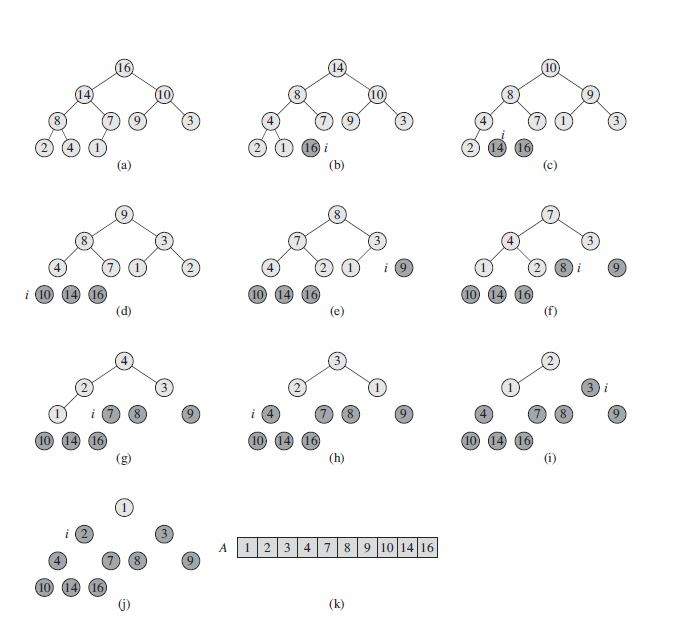
\includegraphics[scale=0.7]{heapsort.jpg}\\
  \caption{Illustration af heapsort}
\end{figure}


\chapter{Binary Search Trees S. 286/308}
\section{Definition}
Et binært søgetræ er et binært træ som skal opfylde visse kriterier.
Hver knude har en nøgle og en associeret værdi og knuder kan højst have op til to børn.
For en knude x, skal der gælde, at en knude y i det venstre undertræ skal have nøgle med samme eller mindre værdi, dvs. y.key $\leq$ x.key, mens der for det højre undertræ skal gælde at en knude y har en nøgle-værdi med samme eller større værdi, dvs x.key $\leq$ y.key.
Hver node antager således at denne pointer til hhv. parent. right eller left-child. I tilfælde der ikke er noget, er det en null pointer.

\section{BST operations and running time}
Det der gør at vi kan printe alle tal ud i en sorteret rækkefølge, kaldes Inorder Tree Walk.
\subsection{Inorder Tree Walk Theroem 12.1}
Hvis x er en rod i et n-node subtræ, kan vi kalde Inorder-Tree-Walk(x) som tager $\Theta(n)$ tid

\textbf{Bevis:}\\
Lad T(n) beskrive tiden det tager Inorder-Tree-Walk. \\
Siden Inorder-Tree-Walk besøger alle n-noder i træet er $T(n) = \Omega(n)$. Vi ved også at T(0) = c for en konstant c > 0.\\
For $n>0$ antag at Inorder-Tree-Walk bliver kaldt på en node $x$ hvor venstre undertræ har $k$ noder og højre har $n-k-1$ noder. Tiden som det tager er begrænset af
\[
T(n) \leq T(k) + T(n-k-1) + d \quad d > 0
\]
Konstanten d skyldes en øvre grænse i det rekursive kald, altså så printer man x.

Vi bruger substitutionsmetoden ved at vise at $T(n)=O(n)$ ved at vise at $T(n) \leq (c + d)n + c$.

For $n = 0$ har vi at $(c + d) 0 = c = T(0)$. For $n > 0$ har vi at
\begin{align*}
  T(n) \leq& T(k) + T(n - k - 1) + d \\
   =& ((c + d) k + c) + ((c + d) (n - k -1) +c ) +d\\
   =& (c + d)n + c - (c + d) + c + d\\
   =& (c + d)n + c
\end{align*}
Således er det vist at $O(n) + \Omega(n) = \Theta(n)$ og dermed slut.


\section{Delete}
Dele operationen har 3 cases. Antag vi kalder delete på element z \textbf{OMFORMULER FØLG BOGEN}
\begin{itemize}
  \item \textbf{z har ingen børn}: Fjerne den. Intet problem, replacer med NIL som barn.\\
  \item \textbf{z har et barn}: Næsten intet problem. Fjern den og lad dens barn tage positionen, ved at ændre relevante pointers.\\
      Altså se billede (a) og (b), hvor z har et barn til højre og et til venstre
  \item \textbf{z har to børn}: Erstart z med den successor y -- som må være i z's højre subtræ -- and og lad y tage z's position i træet. Resten af z's originale højre træ bliver  y's og z's vesntre bliver y's venstre subtræ.\\
      Hvis y ligger i z's højre side og har ingen venstre børn (c), så splicer vi y fra dens nuværende position til at erstatte z. Altså lader man bare y's barn være hvor det er\\
      Hvis y ligger inde i z's højre subtræ, men er ikke z's højre barn (d). Vi bliver først nødt til at erstatte y med dens eget barn og så erstatte z med y\\
%      For at hjælpe med ovenstående defineres i algoritmebogen en subprocedure kaldes Transplant som erstatte en node u med en node v, og sørger for at opdatere pointers barn.\\
%      Med ovenstående definition kan casen med ingen barn håndteres i et enkelt transplant kald (Fordi NIL node tillades i Transplant subproceduren), såvel som både højre og venstre et-barns casen kan løses med et enkelt transplant kald.\\
%      \begin{enumerate}
%        \item Lad y være z's successor
%        \item Hvis: y ikke er barn af z. Transplant y med y.child
%        \item transplant z med y
%      \end{enumerate}
\end{itemize}

køretiden er igen $O(h)$ fordi vi finder successor, som gør brug af minimum

\begin{figure}[H]
  \centering
  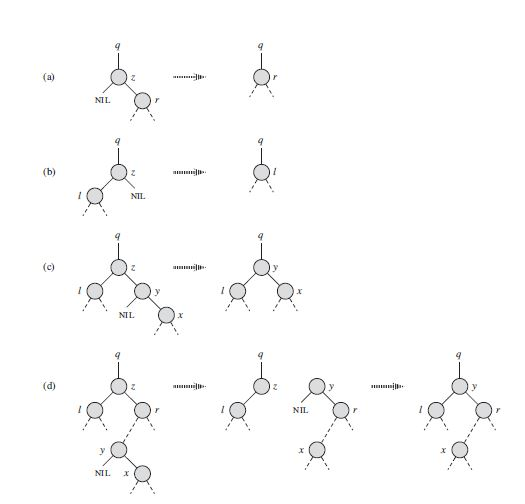
\includegraphics[scale=0.8]{delete.jpg}\\
  \caption{ }
\end{figure}

\section{Red-Black-Trees}
Som det fremgå af gennemgangen af operationerne for Binære søgetræer, så er køretiden afhængig for højden af træet. Jeg vil derfor snakke om Red-Black trees som er løsning på dette problem.
\subsection{Definition}

\begin{enumerate}
  \item Hver node er enten sort eller rød (1)
  \item Roden er sort
  \item Hvert blad er sort (2)
  \item Hvis en node er rød, er begge børn sorte (3)
  \item For hver node, ned til et blad, passeres lige mange sorte noder (4)
\end{enumerate}
\subsection{Lemma 13.1}
Et R-B træ med n interne noder har højst højden $2 \log(n+1)$
Bevis:\\
Hver node har mindst $2^{bh(x)}-1$ noder

Dette bevises ved induktion. Et træ med højde 0 har ifølge basecase mindst $2^0 - 1 = 0$ elementer hvilket passer.\\
Antag en node x med blackheight $bh(x)$ hvert af den børn har en blackheight på enten $bh(x)$ hvis den er rød eller $bh(x)-1$ hvis den er sort\\
Bruger vi induktion kan vi sige at barnet har mindst $2^{bh(x)-1}-1$ interne noder. Node x har dermed i antal noder, udregnet fra børn plus sig selv, dvs.
\begin{align*}
  n  =& 2(2^{bh(x)-1}-1) +1 \\
     =& 2(2^{bh(x)}2^{-1}-1) +1 \\
     =& 2^{bh(x)} - 2 +1 \\
     =& 2^{bh(x)} - 1 \\
\end{align*}

Ovenstående nedre grænse for antallet af nodes i forhold til bh(x) kan vendes om til en øvre grænse for højden ved at isolere bh(x) hvilket giver $\log(n+1)$

Lad h være højden af træet, så ifølge property 4 ved vi at højst halvdelen af nodes fra hver node til et blad kan være sorte. Derved vil black-height fra roden være mindst h/2 og derfor må
\[
h \geq 2^{h/2}-1
\]
hvis man tager logaritmen og flytter 1-tallet til venstre så får man at $h \leq 2 \log(n+1)$

\subsection{Rotation}
\begin{figure}[H]
  \centering
  % Requires \usepackage{graphicx}
  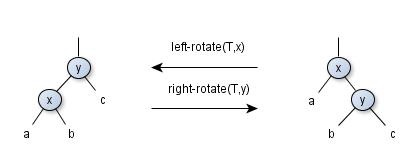
\includegraphics[scale=1]{rota.jpg}\\
  \caption{Rotation O(1)}
\end{figure}
Rotationer bliver brugt  mange stedet til at rebalancere træers højde. Den simple forklaring er .. henviser til billedet.


\subsection{Insertion  S. 315}
Bemærk properties 2 og 4.

Man insætter en rød node og hvis dens parent er rød, violater den red-black properties og man skal køre fixup

Fixup tjekker om onklen er rød eller sort. Derudover bliver der også tjekket om z.p er right eller left child og om z er right eller left child. Basically er der 4 cases

\begin{description}
  \item[case 1] x's onkel er rød
  \item[case 2] x's onkel y er sort og x er højre barn
  \item[case 3] x's onkel y er sort og x er venstre barn
\end{description}

RB-insert(T,x)
\begin{itemize}
  \item indsætter node x og farver den rød (måske en violation)
  \item børn til x er NIL, altså hvis x.p er roden, så er x.p sort
  \item Find en plads i træet til z som er NIL, violater måske property 2 eller 4
  \item O(log n)
\end{itemize}

RB-insert-fixup(T,z)
\begin{itemize}
  \item kører while z.p = red ellers farver den bare T.root sort
  \item Hvis z.p er roden, så startede z.p som sort og der behøves ingen ændringer
  \item Terminates hvis case 2 eller 3 køres
  \item O(log n) fordi man tjekker opad i træet og går ikke ned igen. Højst to rotationer og de tager konstant tid
\end{itemize}

\begin{figure}[H]
  \centering
  % Requires \usepackage{graphicx}
  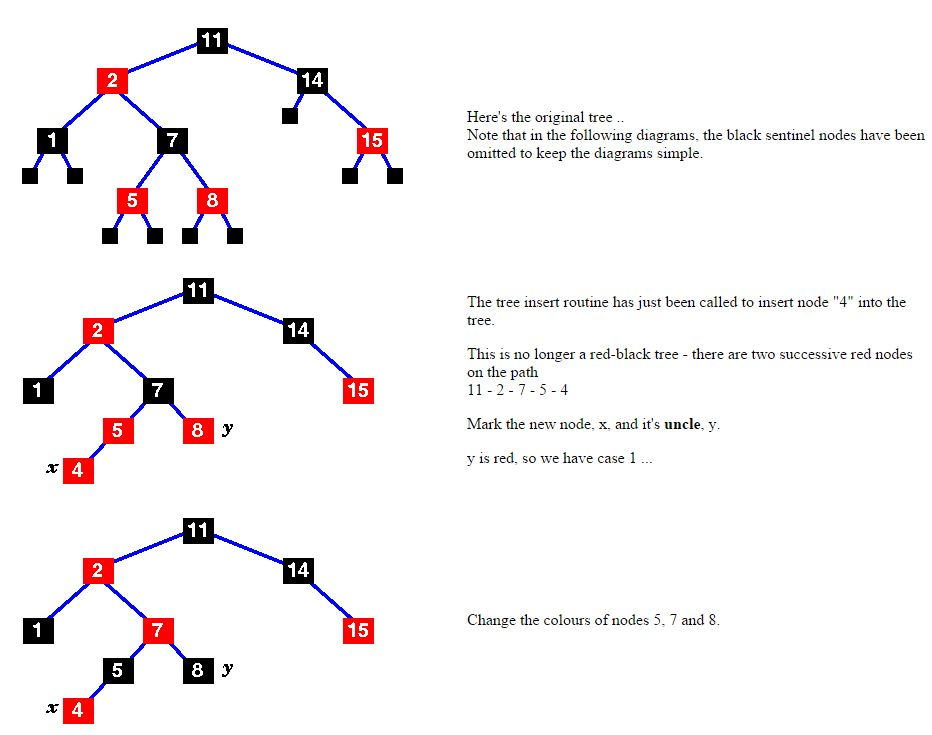
\includegraphics[scale=0.5]{RBInsert1.jpg}\\
  \caption{Illustration af insert}
\end{figure}

\begin{figure}[H]
  \centering
  % Requires \usepackage{graphicx}
  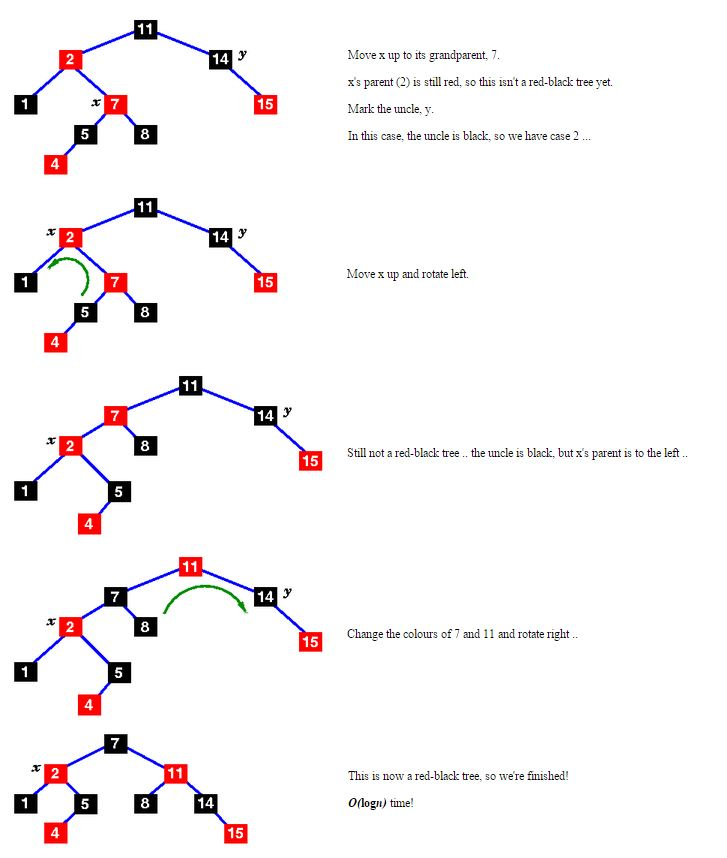
\includegraphics[scale=0.7]{RBInsert2.jpg}\\
  \caption{Illustration af insert}
\end{figure}

\newpage

%\subsection{Deletion S. 323}
%Bemærk properties 1,2, 4 og 5.
%
%Man kan violate blackheight ved at slette en sort node og erstatte den slettede node med en der var sort. Blackheight kan miste en sort node og man skal køre fixup.
%
%Man sletter selve noden på samme måde som ved binary-search-trees
%
%y er en node der bliver slettet eller flyttet i træet, x er noden der overtager z's plads
%
%Hvis node y var sort, kan der opstå 3 problemer
%\begin{enumerate}
%  \item Hvis y var roden, og et rødt child bliver den nye rod, kig på property 2
%  \item hvis x og x.p er røde, så violater vi property 4
%  \item Hvis vi flytter y indeni træet, ved at ændre vejen som y
%\end{enumerate}
%
%køretiden er det samme som i insertion.


\chapter{Dynamic Programming S. 359}
Dynamisk programmering bruges til at løse problemer som kan deles i mindre problemer, men hvor problemerne overlapper. Brugte man Divide and Conquer, ville man løse de samme problemer mange gange.

For at løse et problem med dynamisk programmering, skal en  optimal løsning altså bestå af samme optimale løsninger til samme problem af mindre størrelser.
Man siger problemer har \textbf{optimal substruktur}. Disse problemer kan have mange mulige løsninger, og derved kan en optimal løsning være løsningen frem for at det er den løsning, fordi der ofte kan være flere som er lige så gode.

Ved dynamisk programmering gør man følgede:
\begin{enumerate}
  \item Find strukturen for den optimale løsning
  \item Definer værdien af en optiaml løsning
  \item Beregn den optimale løsning (Fortrinsvis buttoms up)
  \item Konstruer en optimal løsning fra det beregnede
\end{enumerate}

Dog skal subproblemerne være uafhængige for at dynamisk programmering virker. Dvs en løsning til et problem må ikke have indflydelse på hvad værdien af en anden løsning bliver!!.


\section{Memoized}
Det er en måde, hvor man i stedet for at genudregne de samme input for værdier, så cacher vi resultatet for hvert kald og bruger det videre mod fremtidige udregninger


\subsection{Top-down}
Ved at tage verdensherredømmet, så siger man at man vil starte med at overtage USA, hvordan vil dette gøres, det gøres ved at ovetage SydAmerika, hvordan? Brasilien først osv osv
\begin{lstlisting}
1   int Fibonacci(n)
2     {
3       if(n<= 1)
4           return 1
5       else
6           return(Fibonacci(n - 1) + Fibonacci(n - 2))
7     }
\end{lstlisting}

\subsection{Bottom-up}
Løser subproblemer ved deres størrelse og løser dem i størrelses orden, altså de mindste først. Gemmer resultetet. For at udnytte det det med verdensherredømmet, så starter du med at sige at du vil overtage Brasilien, derefter Argentina osv osv.

\begin{lstlisting}
1   int Fibonacci(n)
2     {
3       int fib[]
4       fib[0] = 1; fib[1] = 1;
5
6       for(int i = 2; i<= n; i++)
7           fib[i] = fib[i - 2] + fib[i - 1]
8
9       return fib[n]
10    }
\end{lstlisting}




\section{LCS Theorem 15.1}
Hvis man skal sammenligne strings i DNA, er der interesse i at finde lighederne, hvor det ikke matcher 100\% men hvor man finder, hvilke strings der matcher i en given string.

For strings som skal matches $X=<x_1,x_2,...,x_m>$ og $Y=<y_1,y_2,...,y_n>$ samt LCS af dem begge $Z=<z_1,z_2,...,z_k>$ gælder følgende:
\begin{enumerate}
  \item Hvis $x_m = y_n$, så $z_k = x_m = y_n$ og $Z_{k-1}$ er en LCS af $X_{m-1}$ og $Y_{n-1}$\\
      Altså så er det også med i Z og begge strings kan forkortes til et mindre problem af samme type.
  \item Hvis $x_m \neq y_n$ så $z_k \neq x_m$ medfører det at Z er en LCS af $X_{m-1}$ og $Y$
  \item Hvis $x_m \neq y_n$ så $z_k \neq x_m$ medfører det at Z er en LCS af $Y_{n-1}$ og $X$
\end{enumerate}

For case 1, hvor sidste karakter matcher, så antag vi har X=<ABCA> og Y=<DACA>, siden begge ender med "A", kan vi sige at LCS også ender med "A". Så fjernes A fra X og Y og man kigger på $X_{m-1}=<ABC>$ og $Y_{n-1}=<DAC>$ som bliver til <AC> og ved at tilføje A'et bliver svaret <ACA>. Så hvis $x_m = y_n$ så er $c[i,j]=c[i-1,j-1] + 1$

For case 2,3 Da hverken både $x_m$ eller  $y_n$ kan være LCS og vi ikke ved hvilken en det er, prøver vi begge cases, derved hvis $x_m \neq y_n$ så $c[i,j] = max(c[i-1,j],c[i.j-1])$

\textbf{Step 1:}
\subsection{15.1}

\textbf{Bevis 1:}\\
Hvis $z_k \neq x_m$, så kan vi tilføje $x_m = y_n$ som skal være med i en LCS og tilføje den til vores LCS Z, som er den \emph{longest} common subsequence og få en længere LCS, som nu har længde k+1, hvilket en en kontradiktion, idet det antages Z er en LCS af X og Y. Fordi det må være at $z_k = x_m = y_n$ og $|z_{k-1}| = k-1$ og er en LCS af $X_{m-1}$ og $Y_{n-1}$\\
Vi skal altså bevise at $Z_{k-1}$ er LCS af $X_{m-1}$ og $Y_{n-1}$. Antag der findes en string W som er LCS af $X_{m-1}$ og $Y_{n-1}$ og at denne har længde længere end k-1, altså $|W|>k-1$. Tilføjer vi da $x_m=y_n$ til W får vi en LCS med længde længere end k og dette er en kontradiktion, idet vi antog at vores LCS af X og Y har en længde k.

\textbf{Bevis 2:}\\
Hvis $z_k \neq x_m$ så er Z LCS af $X_{m-1}$ og $Y_n$. Hvis der findes der en string $|W|>k$, så vil W være en LCS af X og Y, hvilket er en kontradiktion igen.

\textbf{Step 2:}
\subsection{Rekursiv løsning}
Vi definere et c[i, j] til at være længden af LCS af sekvensen af $X_i$ og $Y_i$. Hvis enten $i = 0$ eller $j = 0$, så har en af sekvenserne længden 0 og dermed er LCS af længden 0. Vi opskriver den rekursive løsning af LCS ved at lave en rekursion på længden
\[
c(i,j) =
    \begin{cases}
        \begin{array}{c}
            0 \quad \text{hvis } i =  0 \text{ og } j = 0 \\
            c(i-1, j-1) +1 \quad \text{hvis } i,j > 0 \text{ og } x_i = y_j \\
            \max\{c(i-1, j), c(i, j-1)\} \quad \text{hvis } i,j > 0 \text{ og } x_i \neq y_j
        \end{array}
    \end{cases}
\]
Dette giver os muligheden for på øjeblikke at skrive en eksponentiel tids algoritme til at give den korrekte løsning og det gør vi ikke.

\textbf{Step 3:}
\subsection{computing LCS}
Brug eksempel hvor vi har $S_1 = \{A, B, C\}$ og $S_2 = \{B, D, C\}$

Vi ønsker at beregne LCS ved en buttoms up metode. For at gøre dette oprettes en $m \cdot n$  matrix til at gemme løsningerne til subproblemerne. vi kan indsætte værdierne vi kender. Nemlig at ved enten i = 0 eller j = 0 er vores bedste løsning, idet intet er blevet matches. Vi kan så udfylde resten af matrxien ud fra dette. Figur 15.8 s. 395

\begin{figure}[H]
  \centering
  % Requires \usepackage{graphicx}
  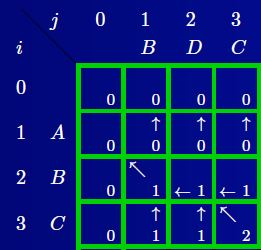
\includegraphics[scale=1]{pile.jpg}\\
  \caption{Illustration af computing LCS}
\end{figure}

\begin{figure}[H]
  \centering
  % Requires \usepackage{graphicx}
  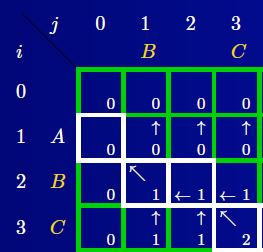
\includegraphics[scale=1]{listedone.jpg}\\
  \caption{Illustration af computing LCS}
\end{figure}

\textbf{Step 4:}
\subsection{The solution}
Man kan undlade at gemme 'pilene' i b og i stedet beregne hvilke 3 elementer $c[i,j]$ blev beregnet vha. Dette gør at man ikke behøver at gemme de $\Theta(mn)$ elementer i b dog bliver man alligevel $\Theta(mn)$ plads til c, så køretiden blev ikke rigtigt ændret.

\section{Bånd til Greedy Algoritmer}
Dynamisk programmering har stærke bånd til Greedy Algortimer. Man kan sige, at greedy algortimer har Dynamisk programmering, hvor det giver en optimal løsning ved hele tiden at tage det valg som ser bedst ud lige nu og her.


\chapter{Greedy Algorithms S. 414}
En grådig algoritme løser problemet ved at gentagne gange løse et subproblem der ser bedst ud på det angivne øjeblik og så løse videre.

\section{Huffman}
Algoritmen fungerer ved at danne et træ, hvor hver encoding starter ved roden af træet. Går man til højrebarnet svarer det til at tilføje et 1-tal til karaktererne tilhørende højre træets encoding bit. Går man til venstre tilføjer man et 0. Hver blad er således en encoding tilhørende en karakter.

Der bliver lavet en effektiv binær kryptering, der bruger så få bit som muligt til en given karaktersæt, med tilhørende frekvenser. Huffman algoritmen sørger for at give de bogstaver med flest forekomster, færrest antal bit til repræsentationen. Samtidig sørger den for at ingen karakters binære repræsentation, er et prefix, til en anden karakter.

Et eksempel kunne være "ABACCDA", hvor
\begin{description}
  \item[A] Optræder 3 gange
  \item[B] Optræder 1 gang
  \item[C] Optræder 2 gange
  \item[D] Optræder 1 gang
\end{description}
Tegn træet og så forklar til sidst bit encoding.

Prisen for et træ B(T) defineres logisk som den expected mean
\[
B(T) = \sum_{c\in C}^{|C|} c.freq \cdot d_T(c)
\]
hvor $d_T (c)$ er dybden for c i træet T, hvilket betyder at hvor mange bits bruges til at encode den pågældne karakter.

Ved at lave Huffman, altså konstruere den, så sætter man $z.freq = x.freq + y.freq$ som det se i eksemplet.

For at bevise at den gråde HUFFMAN algoritme er korrekt, vises dette ved Lemma 16.2

\subsection{Lemma 16.2}
Lad C være et alfabet, hvor hvert bogstav $c \in C$  har en frekvens c.freq, hvor C er et alfabet. Lad x og y (\{x,y\}) være to elementer i C med laveste frekvens. Da findes der et træ T, som repræsenterer en optimal prefix code, hvor x og y er søskende, har maksimal dybde og dermed kun har en forskel i deres sidste bit.

\textbf{Bevis:}\\
Lad \{a,b\} være to søskende på maksimal dybde i træet T. Da gælder at
\[
d_T(x) \leq d_T(a)
\]
\[
d_T(y) \leq d_T(b)
\]
Antag, for bare at vælge noget, at
\[
x.freq \leq y.freq \quad AND \quad a.freq \leq b.freq
\]
Da gælder det også at
\[
x.freq \leq a.freq \quad AND \quad y.freq \leq b.freq
\]

Vi definer nu et $T'$ som $T$ hvor x og a bytter plads. Da vi antager $T$ repræsenterer en optimal Huffman code kan vi skrve prisen for $T'$ ud fra ændringerne til $T$.
Husk at det antages at $T$ er optimal, og det må da gælde at $B(T) \leq B(T')$.

\begin{figure}[H]
  \centering
  % Requires \usepackage{graphicx}
  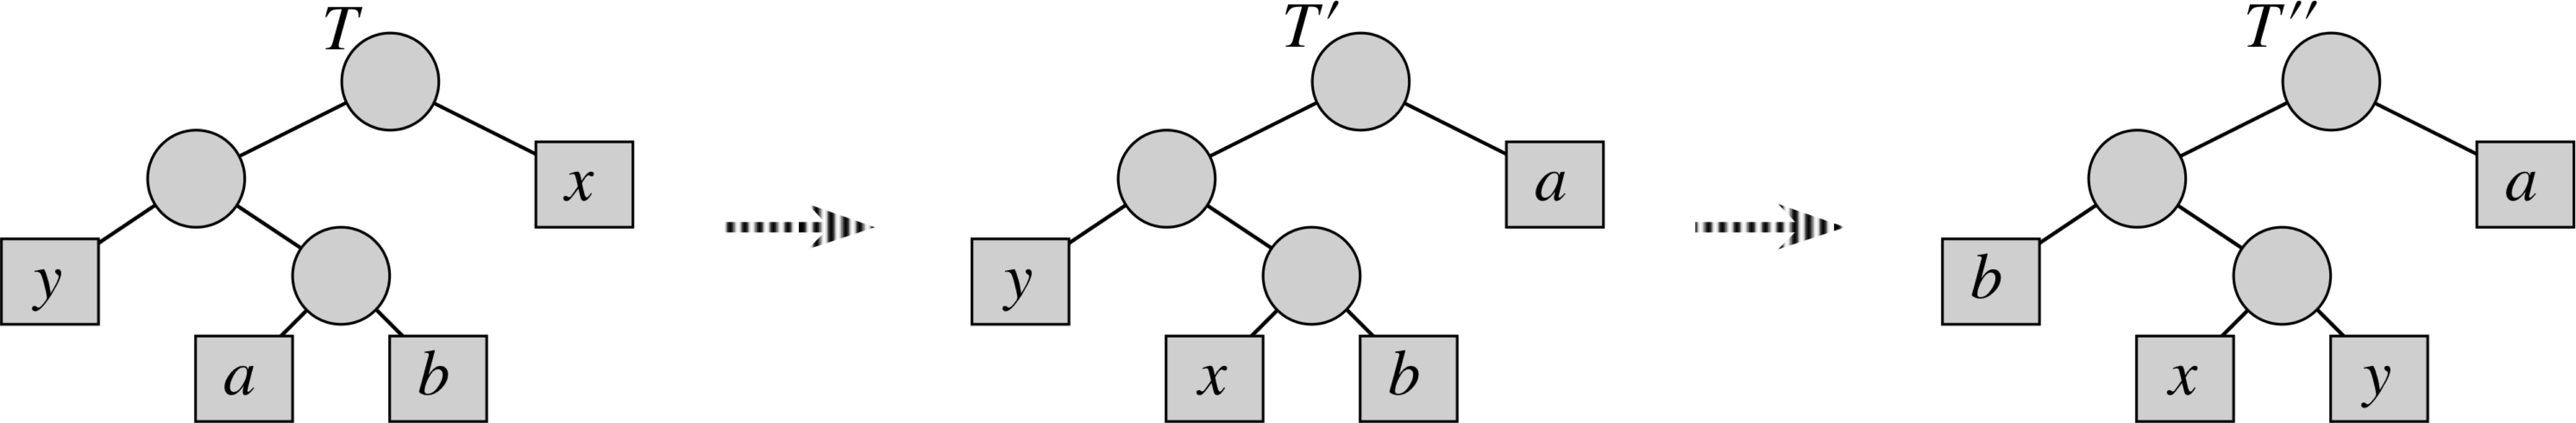
\includegraphics[scale=0.06]{lemma163.jpg}\\
  \caption{Til beviset lemma 16.2}
\end{figure}

\begin{align*}
  B(T) - B(T') =&  x.freq \cdot d_T(x) + a.freq \cdot d_T(a) - x.freq \cdot d_{T'}(x) - a.freq \cdot d_{T'}(a) \\
   =& x.freq \cdot d_T(x) + a.freq \cdot d_T(a) - x.freq \cdot d_T(a) - a.freq \cdot d_T(x) \\
   =& (a.freq - x.freq)(d_T(a) - d_T(x))\\
   \geq& 0
\end{align*}
Dermed er det vist at $B(T) \leq B(T') \leq B(T)$ og dermed at $B(T) = B(T')$.

Samme gælder for y og b, hvor vi har T' og derved får vi at $d_{T''}(y) = d_{T'}(b)$ og $d_{T''}(b) = d_{T'}(y)$ og samme udregninger fås, hvor man så har $B(T') - B(T'') = B(T') \leq B(T'')$

Altså er det vist at ved at bygge et optimalt træ, kan man tillade sig at være grådig og merge to træer sammen med hvilken karakter har lavest frekvens

Nu vises at der er optimal substructre property

\subsection{Lemma 16.3}
Lad C være et given alfabet med frekvens c.freq defineret for hver karakter $c \in C$. Lad x og y være to karakterer i C med mindst frekvens.\\
Lad C' være det alfabet med karakterne x og y fjerne men z tilføjet, altså $C' = C - \{x,y\} \cup \{z\}$ hvor $z.freq = x.freq + y.freq$ hvor et træ $T'$ som dannet fra T ved at bytte den node som x og y deler ud med z, repræsenter optimal prefix code for $C'$.

\textbf{Bevis:}\\
Først vises kosten af B(T) af træet T, ud fra kosten af B(T') af træet T'. For hver karakter $c \in C - \{x,y\}$ har vi at $d_T(c) = d_{T'}(c)$ og siden $c.freq \cdot d_T(c) = c.freq \cdot d_{T'}(c)$ og siden $d_T(x) = d_T(y) = d_{T'}(z) +1$ har vi at $x.freq \cdot d_T(x) +y.freq\cdot d_T(y)$. Altså
Da
\[
d_T(x) = d_T(y) = d_{T'}(z) +1
\]
så kan vi komme frem til at
\begin{align*}
  x.freq \cdot d_T(x) + y.freq \cdot d_T(y) = & (x.freq + y.freq)(d_{T'}(z) +1) \\
  =& z.freq \cdot d_{T'}(z) + x.freq + y.freq
\end{align*}

dermed må det gælde at

\begin{align*}
  B(T)  =& B(T') + x.freq + y.freq \\
  B(T') =& B(T) - x.freq - y.freq
\end{align*}

Nu bevsises det ved brug af kontradiktion

\begin{enumerate}
  \item Antag T ikke repræsenterer en optimal prefix code til C. Der må dermed eksistere et træ som repræsentere et optimalt træ $T''$ og dermed $B(T'') < B(T)$
  \item pga lemma 16.2 har $T''$, x og y som søskende
  \item Definer $T'''$ som $T''$ hvor x og y byttes med z
\end{enumerate}
Da gælder at
\begin{align*}
  B(T''') =& B(T'') - x.freq - y.freq \\
  < & B(T) - x.freq - y.freq \\
  = & B(T')
\end{align*}
$T'$ antages for at være optimal. Ovenstående viser, at hvis man prøver at antage at T ikke er optimal, da vil $T'$ pludselig heller ikke være optimal. Dermed må T være optimal.

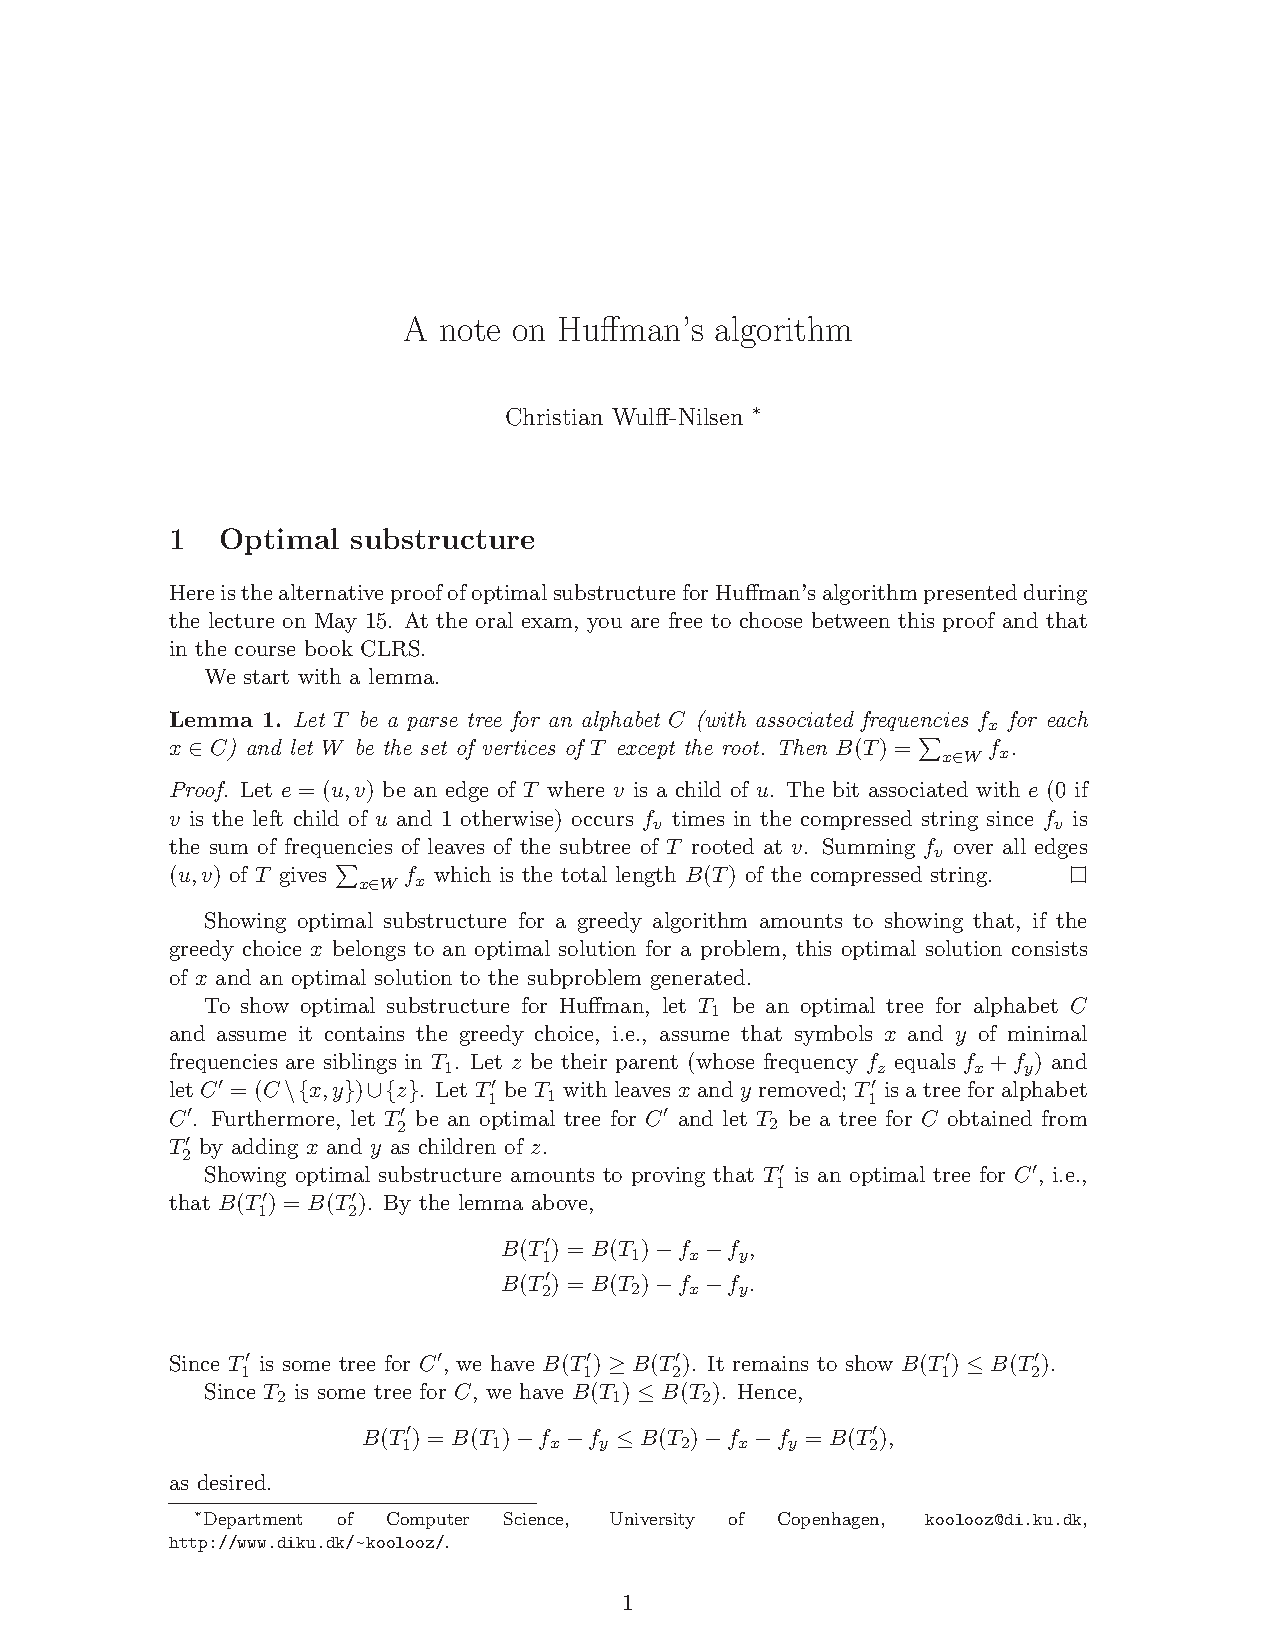
\includepdf{notes.pdf}

\chapter{Minimum Spanning Trees S. 624}

Man kan lave en model hvor vi har en graf $G = (V, E)$ hvor
\begin{itemize}
  \item V: Knuder i grafen og deres værdier
  \item E: er kanter i grafen $(u, v)$, altså $(u, v) \in E$
  \item w: er en funktion der returnerer vægten af en kant, w(u,v), altså hvad det koster at forbinde u og v.
\end{itemize}
Den totale vægt kan defineres som $w(T) = \sum_{(u,v)\in T} w(u,v)$.

Antag at vi har en graf G=(V,E) med vægt funktion $w:E\rightarrow \mathbb{R}$ og vi ønsker at finde MST for G.  Så er A er et subset til et MST for G, lad (S, V-S) været et cut af G som respekterer A, altså ikke deler indre kanter i A, da vil den kant, (u, v), med den mindste værdi være sikker at tilføje til A. Så til hvert skridt til når man skal besteme en kant (u, v) som kan tilføjes til A, kan det skrives som $A\cup \{(u,v)\}$

\section{Theorem 23.1}

\begin{figure}[H]
  \centering
  % Requires \usepackage{graphicx}
  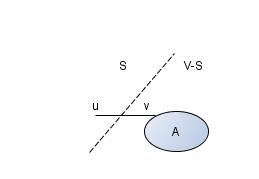
\includegraphics[scale=1]{MSTcut.jpg}\\
  \caption{Figur 23.3}
\end{figure}

Lad G=(V, E) med $w:E\rightarrow \mathbb{R}$ defineret på E. Lad A være et subset af E som er inkluderet i G som er et MST.
Givet et (S,V-S) cut som respekterer A (ikke deler indre kanter i A). Da vil den kant (u,v) som har den mindste værdi være sikker på at tilføje til A (således at A stadig er inkluderet i et MST).

\textbf{Bevis:}\\
Lad T være et MST som inkluderer A. Antag at (u, v) ikke er med i vores MST T. Siden (u, v) ikke er inkluderet i MST, må der være en anden simpel rute fra u til v. Denne rute er nødt til på et tidspunkt at krydse vores cut (S, V-S).\\
Lad (x,y) være denne kant.

\begin{figure}[H]
  \centering
  % Requires \usepackage{graphicx}
  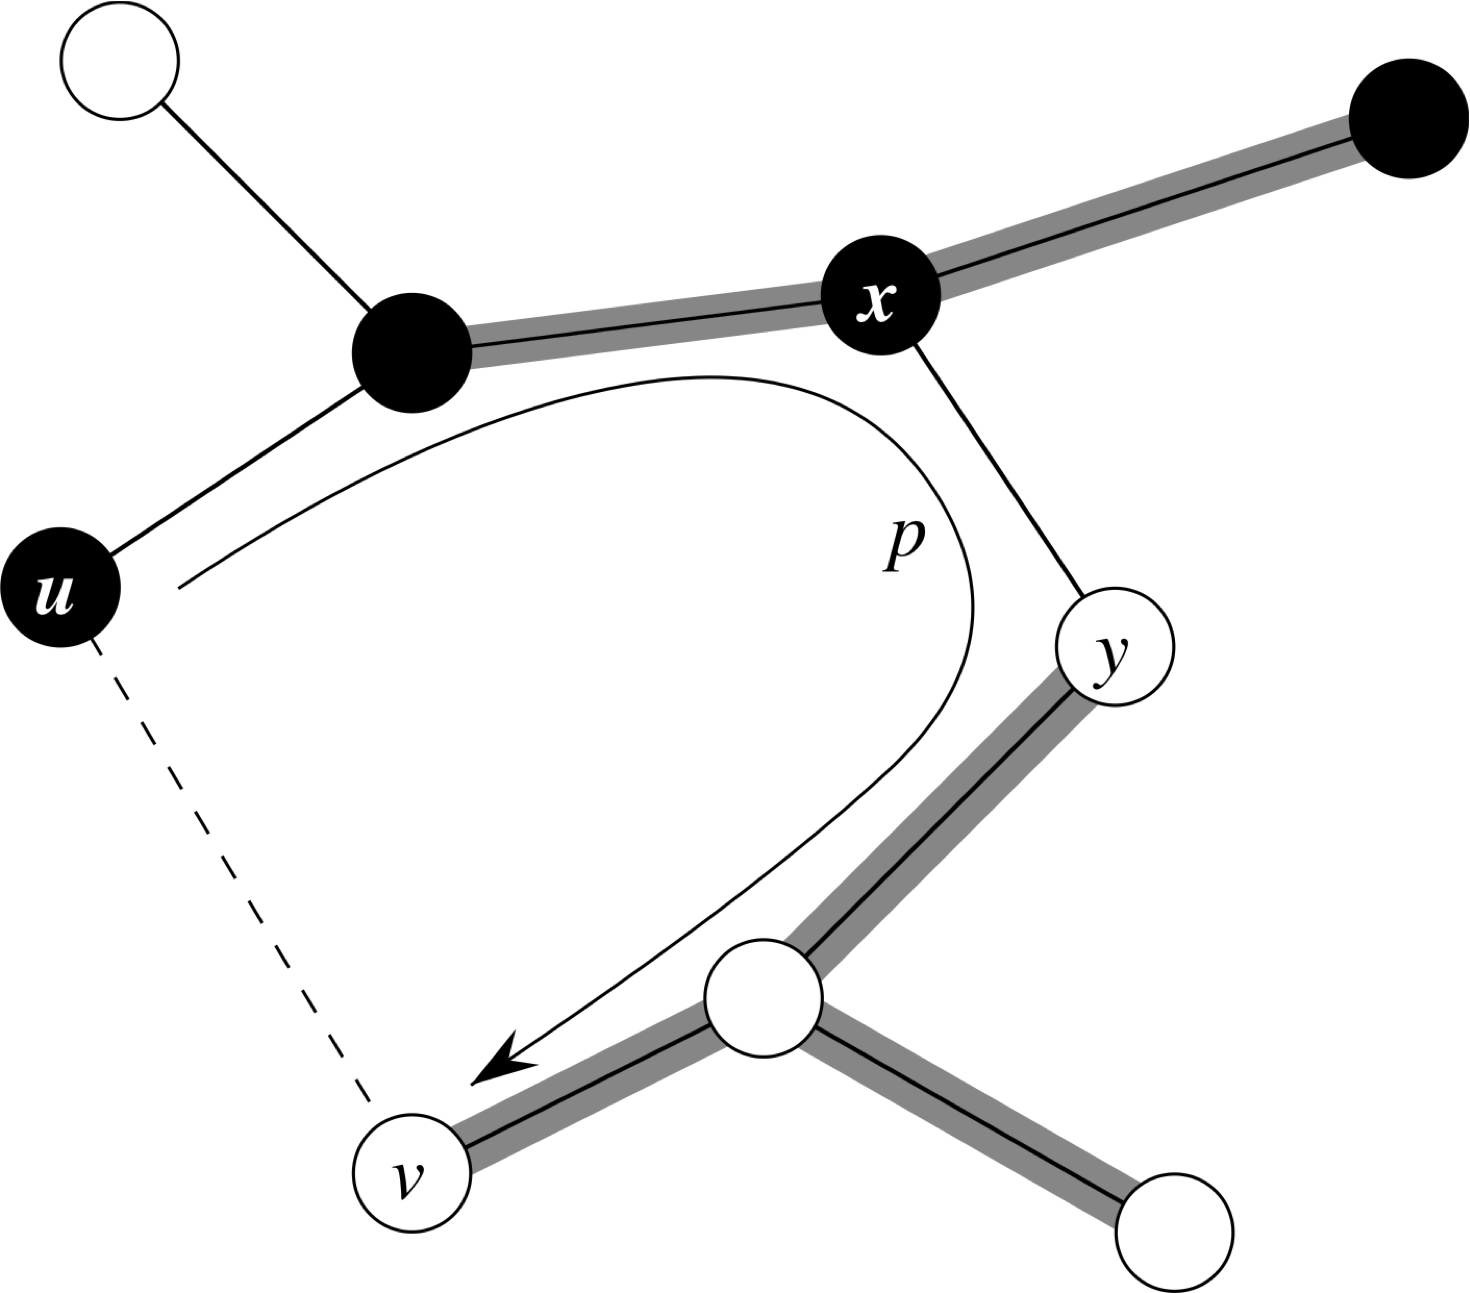
\includegraphics[scale=0.15]{figur233.jpg}\\
  \caption{Figur 23.3 hvor de hvide kanter er i V-S og de sorte er i S}
\end{figure}
Altså at $A\in T$ og at $(u,v)\notin T$. Vi kan nu definere et nyt træ $T' = T - \{(x,y)\} \cup \{(u,v)\}$. Vi ved at $w(T) \leq w(T')$ og $w(u,v) \leq w(x,y)$. .  Prisen for $T'$ er da:
\begin{align*}
w(T') =& w(T) - w(x,y) + w(u,v) \quad \text{Da } (- w(x,y) + w(u,v)) \text{ er } \leq 0 \\
 \leq & w(T)
\end{align*}
Men da T er et MST, således at $w(T) \leq w(T')$; må T' også være et MST
\[
(u,v) \text{ \textbf{er sikker på at tilføje til A:}}
\]
Fordi $A \subseteq T'$, fordi $A \subseteq T$ og $(x,y) \notin A$ men tilgengæld er $A \cup \{(u,v)\} \subseteq T'$. $T'$ er et MST, da må $(u,v)$ være sikker på at tilføje for A


\section{Kruskal}

\begin{lstlisting}
1   A = EMPTY
2   for each vertex v IN G.V
3     MAKE-SET(v)
4   sort the edges of G.E into nondecreasing order by weight w
5   for each edge (u,v) \in G.E, taken in nondecreasing order by weight
6     if FIND-SET(u) != FIND-SET(v)
7       A = A UNION {(u,v)}
8       UNION(u,v)
9   return A
\end{lstlisting}

1-3 initialisere sættet A til et tomt sæt og laver $|V|$ træer\\
For-loopet tjekker om kanterne i forhold til vægten, fra lav til høj og loopet tjekker for hver kant (u,v), om slutenderne u og v er i samme træ.\\
7 tilføjer kanten (u,v) til A.\\
8 mergert kanterne sammen til to træer.

Eksempel på Kruskal med graf og tegn (Running time)\\
Holder alle vertex forbåndet fra source og følger den mindste

Med FIND-SET, UNION operationer og med $|V|$ MAKE-SET operationer, så tager den totale køretid på dette $O((V+E)\alpha(V))$, hvor $\alpha$ er en langsom voksende funktion. Da vi antager at G er forbåndet, har vi $|E| \geq |V| -1$ og dette tager $O(E \alpha(V))$ tid, da $\alpha(|V|) = O(lg V) = O(lg E)$ og ved at obsverer at $|E| < |V|^2$, så er den totale køretid O(E lg V)

\section{Prims algoritme}

the connected graph G and the root r of the MST to begrown are inputs to the algorithm. During the execution of the algorithm, all vertices that are not in the tree reside in a min-priority queue Q based on the key attribute. For each vertex v, the attribute v.key is the minimum wieght of any edge connectring v ot a vertex in the tree; by convention, v.key = $\infty$ if there is no such edge. the attribute $v.\pi$ names the parent of v in the tree.

\begin{lstlisting}
1   for each u IN G.V
2     u.key = infinity
3     u.PI = NIL
4   r.key = 0
5   Q = G.V
6   WHILE Q != EMPTY
7     u = EXTRACT-MIN(Q)
8     for each v IN G.Adj[u]
9       if v IN Q and w(u,v) < v.key
10        v.pi = u
11        v.key = w(u,v)
\end{lstlisting}

Linie 1-5 sætter hver key til hver vertex til $\infty$ udover root, r, som sættes til 0.\\
Linie 6-11
\begin{enumerate}
  \item $A = \{(v,v.\pi) : v \in V - \{r\} - Q \}$
  \item The vertices already placed into the MST are those in V - Q
  \item For alle vertices $v \in Q$, if $v.\pi \neq $ NIL, then $v.key < \infty$ and $v.key$ is the weight of a edge $(v,v.\pi)$ connecting v to some vertex alreadyt placed into the minimum spanning tree
\end{enumerate}

Linie 8 identificerer en vertex $u \in Q$ som krydser (V-Q,Q)

Eksempel på Prim med graf og tegn (Running time)
Tager altid den mindste vertex

Prim's algoritme fungerer på samme vis som Dijkstra Short Path algoritme, idet den bygger et minimum spanning tree op ved at vælge billigste rute fra en besøgt knude til en ubesøgt knude, for ved hver iteration at tilføje en knude til det MST man er ved at bygge på.\\
Køretiden er meget afhængig af hvilken datastruktur som bruges. En min-heap priority queue kan bruges. Den skal først bygges hvilket gøres i $O(V)$ tid. Hver knude skal udtrækkes ved $Extract-Min$ operationen hvilket gøre i $O(V \log V)$ tid. Dog skal man potentielt opdatere alle værdiere af knuder som har en edge der møder en inkluderet knude. Dette skal potentielt gøres E gange og tager $O(\log V)$ tid asymptotisk. Derfor bliver en totalte køretid $O(E \log V)$ tid, som er det samme som Kruskal (lemma 23.1)

\chapter{Shortest Path S. 684}
\begin{itemize}
  \item V: Knuder i grafen og deres værdier
  \item E: er kanter i grafen $(u, v)$, altså $(u, v) \in E$
  \item w: er en funktion der returnerer vægten af en kant, w(u,v), altså hvad det koster at forbinde u og v.
\end{itemize}

hvor vægten af $w(p)$ af pathen $p = \langle v_0, v_1, ... , v_k \rangle$ er summen af dens vægte
\[
w(p) = \sum^k_{i=1} w(v_{i-1},vi)
\]
således definere vi den korteste vejs vægt $\delta(u,v)$ fra u til v med
\[
\delta(u,v) =
\begin{cases}
              \begin{array}{c}
                min\{w(p):u \leadsto^{p} v\}, \quad \text{from u to v } \\
                \infty, \quad \text{otherwise}
              \end{array}
              \end{cases}
\]


\begin{itemize}
  \item $v.d$ - længden af den nuværende korteste vej fra $s$ til $v$. Dette er initialiseret til at være $\infty$ for alle knuder udover source knuden og de bliver mindre hen af vejen når man finder kortere og kortere vej. Til slut vil dette være vægten af den korteste vej, hvor s.d er initialiseret til at være 0
  \item $v.\pi$ Predecessor af v i den SP fra s til v
  \item $w(u,v)$ er vægten af en kant fra en knude $u$ til en knude $v$
  \item $\delta(u,v)$ er længden af den korteste vej fra knude $u$ til knude $v$
\end{itemize}


\section{lemma 24.1}
Givet en vægtet, graf $G=(V,E)$ med $w : E \rightarrow \Real$, lad $p = \langle v_0, v_1, ... , v_k \rangle$ være den korteste vej fra et vertex $v_0$ til vertex $v_k$ og for et abitrært i og j således at $0 \leq i \leq j \leq k$ lad $p_{ij}= \langle v_i, v_i+1, ... , v_j \rangle$ være subvejen af p fra vertex $v_i$ til $v_j$. Så er $p_{ij}$ den korteste rute fra $v_i$ til $v_j$.

\textbf{HUSK:} Givet en graf $G=(V,E)$ ønskes der at findes en korteste vej fra en given "source" knude $s\in V$ for hver knude $v \in V$

\section{Relax}
For hver knude $v \in V$ beholder vi at $v.d$ som er en upper bound på vægten af den korteste vej fra source s til v. Genkend at $v.d$ er shortest-path estimate. Vi initalisere den korteste vej med tid $\Theta(V)$.\\
Efter initialisationen har vi at $v.\pi = NIL$ for alle $v\in V, s.d = 0, v.d = \infty$ for $v \in V - \{s\}$

Ved start af algoritmen så sætter man $v.d$ til $\infty$ og $v.\pi$ til NIL. Med tiden som algoritmen kører, opdateres disse værdier til at finde den korteste vej.\\
Ideen er at hvis vi finder en vej der koster $u.d$ fra $s$ til $v$ og der er en kant fra $u$ til $v$, så er den øvre grænse på vægtkosten af den korteste vej fra $s$ til $v$ nemlig $u.d$ plus vægten fra kanten mellem $u$ og $v$. Vi kan sammenligne $u.d + w(u,v)$ med $v.d$ og opdater $v.d$ hvis $u.d + w(u,v)$ er mindre end den nuværende $v.d$.

\begin{lstlisting}
RELAX(u, v):
  if v.d > u.d + w(u, v) // if we find a shorter path to v through u
    v.d = u.d + w(u, v) // update current shortest path weight to v
    v.pi = u // update parent of v in current shortest path to v
\end{lstlisting}

\section{Bellman-Ford Algoritmen s. 651}
Bellman-Ford løser single-source shortest-path problemerne hvor kanternes vægt kan være negativ.
Initializationen tager $\Theta(V) $ tid. Hver af de $|V|-1$ passeringer af kanterne tager $\Theta(E) $ tid og at tjekke for negative cykler tager $O(E)$ tid, altså er køretiden $O(V E)$.

\subsection{lemma 24.2}
Lad $G=(V,E)$ være en vægtet graf med start, s og vægtningsfunktion $w: E \rightarrow \mathbb{R}$ og antag at $G$ indeholder ingen negative vægts-værdier som kan nås fra s.\\
Efter $|V|-1$ iterationer af Bellman-Ford har vi at $v.d = \delta(s,v)$ for alle knuder (vertices) som kan nås fra s, altså er der lavet en shortest path.

\textbf{Bevis}:\\
Så derved for alle $v \in V$ er der en vej fra s til v hviss BF terminates med $v.d\leq \infty$

Antag der er en vej fra s til v, altså $p=\langle v_0, v_1,...,v_k \rangle$, hvor $v_0 = s$ og $v_k = v$ Da p at most har $|V| - 1$ kanter, så er $k \leq |V| - 1$ ender vi med at pga relaxation at $v.d = \delta(s,v) < \infty$

Derved antag igen at BF-terminates med $v.d < \infty$ og på Ubber-Bound property så $d(s,v) \leq v.d < \infty$ og således er der en vej fra s til v.

\subsection{correctness 24.4}
Lad $G=(V,E)$ være en vægtet graf med start, s og vægtningsfunktion $w: E \rightarrow \mathbb{R}$.

Hvis G ikke indeholder nogen negative værdier som kan nås fra s, så returner vi TRUE, vi har $v.d=\delta(s,v)$ for alle knuder (vertices) $v \in V$ og den forgående delgraf $G_{\pi}$ er den korteste rute på s.

Hvis G indeholder negativer værdier så returneres der FALSE.

\textbf{Bevis}:\\
Antag G ikke har nogen reachable negative vægts cykluser fra source s, så for $v\in V$ hvis v er reachable så $v.d = \delta(s,v)$ og hvis ikke så $v.d = \delta(s,v) = \infty$.

Bellman-Ford returnere TRUE når $v.d\leq v.d + w(u,v)$ for alle kanter $(u,v)\in E$, derved
\begin{align*}
  v.d =& \delta(s,v) \\
  \leq & \delta(s,u) + w(u,v) \quad \text{af trekantsuligheden} \\
  =& u.d + w(u,v)
\end{align*}
som returner TRUE

Antag nu at G inderholder negative værdier der kan nås fra source, s; let denne cyklus være $c=\langle v_0, v_1, ... ,v_k\rangle$, hvor $v_0=v_k$. Så har vi at
\[
w(c) = \sum_{i=1}^{k} w(v_{i-1},v_i) < 0
\]
Antag nu, med formål af modstrid at Bellman-Ford algoritmen returner TRUE. Derved $v_i .d \leq v_{i-1} .d + w(v_{i-1}, v_i)$ for $i=1,2,...,k$ og ved at summerere ulighederne om cyklus c, giver os
\begin{align*}
  \sum_{i=1}^{k} v_i .d \leq& \sum_{i=1}^{k} (v_{i-1}.d + w(v_{i-1},v_i)) \\
  = & \sum_{i=1}^{k} v_{i-1}.d + \sum_{i=1}^{k} w(v_{i-1},v_i) \geq 0 \quad \text{Hvilket er en modstrid}
\end{align*}
siden $v_0=v_k$, så har vi at
\begin{align*}
  \sum_{i=1}^{k} v_{i-1} .d =  & v_0 + v_1 + ... + v_{k-1} \\
  = & v_k + v_1 + ... + v_{k-1}\\
  = & \sum_{i=1}^{k} v_{i} .d
\end{align*}
og ved korollar 24.3, er $v_i.d$ endelig for $i=1,2,...,k$, altså
\[
0\leq \sum_{i=1}^{k} w(v_{i-1},v_i)
\]
Som giver en modsigende ulighed. Altså er der modstrid!!

Vi kan konkludere at Bellman Ford algoritmen returnerer TRUE hvis grafen G indeholder ingen negative værdier som kan nås fra start ellers FALSE.


\section{Dijkstra Algoritme s. 658}
Man extracer den minimale knudeværdi og så relaxer man dennes knudes naboer. Så extracter man igen den minimale knudeværdi osv. Der relaxes i tilfældig rækkefølge.

\subsection{correctness 24.6}
Vi ønsker at vise at $u.d = \delta(s,u) $ $\forall u \in V$ når Dijkstra's algortime terminerer.

Loop invariant: Før hver iteration gælder $v.d = \delta(s, v) : \quad \forall v \in S$.

\begin{figure}[H]
  \centering
  % Requires \usepackage{graphicx}
  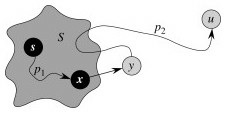
\includegraphics[scale=1]{dijkstra.jpg}\\
  \caption{$u\neq s$}
\end{figure}



\textbf{[INIT]}\\
Trivielt da S = $\emptyset$

\textbf{[MAIN]}\\
Vi ønsker at vise at for hver iteration $u.d=\delta(s,u)$ for knuden tilføjet til sættet S.

For modsigelsens skyld, Lad $u$ være den næste knude som bliver tilføjet og at $u.d \neq \delta(s,u)$ når det bliver tilføjet til sættet S

Vi må derfor have at $u \neq s$ fordi s er den første knude til sættet S og $s.d=\delta(s,s)=0$ på det tidspunkt. Da $u\neq s$ så har vi også at $S\neq \emptyset$ før u er tilføjet til S. Der må være en vej fra s til u for ellers har vi at $u.d=\delta(s,u)=\infty$ af no-path property, som vil være mod vores antagelse at $u.d\neq \delta(s,u)$. Da der mindst er en vej, så er der en korteste vej "p" fra s til u.  Lad "hoppet" være fra knude x til en knude y. Lad $x\in V$ og $y\in V-S$, hvor x er y's predecessor langs "p". Derfor kan vi nu langs "p" dekopmonere en rute ($p_1(s,x)$, $(x,y)$, $p_2(y,u)$) altså $s \rightsquigarrow^{p_1} x \rightarrow y \rightsquigarrow^{p_2} u$.

Altså påstår vi at $y.d = \delta(s,y)$ når $u$ er tilføjet til S. Observer at $x \in S$, så da vi valgte u til at være den første knude som er $u.d\neq \delta(s,u)$, når tilføjet til S, har vi at $x.d=\delta(s,x)$ når x er tilføjet til S.

Da x i sin tid blev tilføjet til S blev kanten (x,y) relaxed og fra konvergensegenskaben er $y.d = \delta(s,y)$.

Vi kan nu vise ved modsigelse at $u.d=\delta(s,u)$, da y kommer før u i den korteste vej fra s til u og alle vægte er ikke negative, har vi at $\delta(s,y)\leq\delta(s,u)$ og derfor har vi
\begin{align*}
  y.d = & \delta(s,y) \\
  \leq & \delta(s,u) \\
  \leq & u.d \quad \text{pga. upper bound property}
\end{align*}

Men da både u og y er i V-S, så har vi at $u.d\leq y.d$, derved får vi at
\[
y.d = \delta(s,y) = \delta(s,u) = u.d
\]

\textbf{[TERM]}\\
Ved $Q = \empty$ som ved vores tidligere invariante ved vi at $Q = V-S$ som betyder at $S = V$. Dermed er $u.d = \delta(s,u)$ for alle knuder $u\in V$


\section*{Bellman-Ford vs Dijkstra}
Den største forskel er at Bellman-Ford kan håndtere negative værdier(vægte) hvor i mod at Dijkstra ikke kan.

\textbf{Single source shortest paths:}

Dijkstra Algorithm - No negative weight allowed - $O(E+Vlg(V))$\\
Man følger den mindste vægt

Bellman ford Algorithm - Negative weight is allowed. But if a negative cycle is present Bellman ford will detect the -ve cycle - $O(VE)$\\
Rækkefølgen er ligemeget

\newpage
\textbf{Hvad der forventes at blive fremlagt til hvert emne
}

1. Del \& hersk\\
 • Eksempel på del og hersk algoritme (ente mergesort eller closest pair)\\
 	Hvorfor er mergesort en del og hersk algoritme?\\
 	Køretid: T(n) = T(ciel(n/2)) + T(floor(n/2)) + cn\\
 	Recursionstræ\\
 	Substitutionsmetoden - det er okay at runde ned begge steder.\\
 • Tal om nedre grænse for comparison-based sorteringsalgoritmer. n lg(n)\\

2. Hobe og prioritetskøer\\
 • Max-hob-egenskaben (en forældres værdi er mindst barnets værdi)\\
 	array-repræsentation\\
 	hvis der er tid: parent, left og right\\
 • Build-max-heap (vis korrekthed og køretid O(n))\\
 • Max-heapify\\
 • Heapsort\\
 • Hvorfor går vi baglæns gennem arrayet? (Krav på max-heapify)\\

3. Balancerede binære søgetræer\\
 • Definer følgende\\
 	Definition på binære søgetræ\\
 	Operationer: Insetion, søg og slet\\
 		Hav et eksempel parat til sletning\\
 • Rød-sorte-træer\\
 	Definition: De 5 betingelser\\
 		Den sorte højde + formål: holde træet i balance\\
 	Bevis for, at højden er begrænset af O(lg(n)), dvs. h <= 2lg(n+1)\\
 		Induktion i højdre - IKKE den sorte højdre\\
 	Operationer: Omfarvning, rotation, insertion og deletion\\
 		Løser problemer ved rotation og omfarvning lokalt og evt. propagerer det op til roden.\\
 		Tal IKKE om det forskellige tilfælde for insert og delete.\\

4. Dynamisk programmering\\
 • Definer og tal om begreberne\\
 	Overlappende delproblemer: Hurtigt fibber-eksempel\\
 	Optimal delstruktur\\
 • Rod-cutting eller LCS - helst LCS, da der er mere kød på denne.\\
 	Vigtigt med konkret eksempel: Skriv to strenge op og opskriv LCS for disse.\\
 	Indfør notation før Lemma!\\
 	LCS Lemma for optimal delstruktur - lemmaet skal bevises\\
 	Opskriv rekursionsformel på baggrund af optimal delstruktur\\
 	Håndkørsel med tabel (3, maks 4 tegn i strengene)\\
 	Køretid og plads for LCS-algoritmen\\
 	Omtal bottom-up (aktuelt eksempel) og memoization\\
 	Hvis der er tid:\\
 		Pladsbesparende version (kun to række, dvs. O(m+n) plads)\\
 		Denne kan dog ikke rekonstruere strengen efterfølgende.\\

5. Grådige algoritmer\\
 • definer og omtal\\
 	Greedy-choice-property: Sig følgende: "Der findes en optimal løsning, der indeholder det grådige \\ valg"
 	Optimal delstruktur Sig følgende: "Hvis vi har en optimal løsning, der indeholder det grådige valg, så består den af det grådige valg plus en optimal løsning til delproblemet"\\
 • Vælg helst strengkomprimering (ellers activity selection)\\
 	Definer problemet\\
 	Konkret eksempel med frekvenser\\
 	Definer B(T): Længde af komprimeret tekststreng\\
 	Problem: Find T, der minimere B(T).\\
 	Hurtig kåndkørsel\\
 	Vis køretid af Huffman (benytter min-hob)\\
 	Korrekthed:\\
 		1) Greedy-choice-property\\
 		2) Optimal delstruktur\\

EVT: Activity selection (bare drop det, da der er mest kød på Huffman)\\
	Opskriv rekursionsformel\\
	Håndkørsel af grådige algoritme\\
	Greedy-choice-property + optimal delstruktur\\

 • Sammenligning med dynamisk programmering\\

6. Mindste udspændende træer\\
 • Definer:\\
 	Definer problemet\\
 	Definition på træ.\\
 	Snit\\
 	Snit som respekterer en delmængde af kanterne\\
 • Den generiske algoritme\\
 	Bevis korrekhed\\
		Vælg lette kant og tilføj til løsning\\
		Opstil løkkeinvariant\\
		Benyt til bevis af korrekthed (mest essentielle i emnet)\\
 • Prim og/eller kruskal\\
 	Datastruktur + køretid\\
 	Husk at vise, hvorfor de er korrekte (de er specialtilfælde af den generiske algoritme)\\
 	Hav et eksempel parat.\\

7. Korteste veje\\
 • Definition:\\
 	Relaxation\\
 • Belmann ford\\
 	Hav eksempel parat\\
 	Bevis korrekthed\\
 	Antal ingen negative kredse (Negative weight cycles)\\
 	Argument for n - 1 iterationer\\
 • Dijkstra\\
 	Bevis korrekthed\\


\end{document} 